%POLAR COORDINATES
% licensed under CC-BY-SA
%% based on: http://www.texample.net/tikz/examples/polar-coordinates-template/ by Zoran Nikolic


%The print template for A4 paper (portrait)
%Author: Zoran Nikolic
\documentclass[10pt]{article}
\usepackage[margin=0.5in,paper=letterpaper]{geometry} %Shrinking margins to 0.5in
\usepackage[x11names,rgb]{xcolor}                     %Additional colors
\usepackage{tikz}
\usetikzlibrary{calc}
\usepackage{euler}                                %Nicer numbers
\usepackage{tkz-base}
\usepackage{tkz-euclide}
\usetkzobj{all}

%Note about the colors: 
%  The color of the "ray" lines should not be
%  black or gray as on some printers, significant
%  aliasing distorsion becomes visible.

\begin{document}
\thispagestyle{empty}
\begin{center}
  {\Large The SubNet Wheel}\\
\end{center}

\section{Subnetting}

An alternate method of subnet visualization can be based on a wheel. The wheel
is broken into $256$ subdivisions where a value is addressed by
$\theta=n_{bits}*360/256$. Basic fomulas for network values are found by:

\begin{tabular}{ll}
Host bits:   	& $h$\\
Network bits: 		& $n=32-h$\\
Number of hosts: 	& $2^h-2$\\
Increment: 		& $2^{n \bmod 8}$ or $2^{8-h \bmod 8}$\\
Netmask: 		& $2^8-2^{n \bmod 8}$\\
\end{tabular}

Applying the CIDR values of $n$ from $24\cdots32$, the diagram shows that the
increment decreases by powers of two from $128$ when viewing the black and white
arc-regions, starting from the origin. It also shows that each increasing CIDR
value is derived by dividing every region in half, following the colord regions,
counter-clockwise. So a $/24$ subnet holds the whole circle, while a $/25$
subnet contains two regions between $0-128$ and $129-255$.

\section{Binary}

Also included in the chart is a binary conversion for the 8 significant bits
within this octet. Bits are read from the outside in.

(Simplified version of the chart shows 7 bits. The last bit is implied by the
even/oddness of the number)

\begin{center}

\begin{tikzpicture}[scale=1.00]

  % draw the sections
  \foreach \t [evaluate = \t as \tfrac using \t/8] in {0,...,7}
  {
    % to rotate through the colors
    \definecolor{fillc}{hsb}{\tfrac,.5,1}
    % to draw the slices
    %\draw [fill=fillc] (0,0) -- ({1.40625*2^\t}:{8-\t}) arc ({1.40625*2^\t}:{1.40625*2^(\t+1)}:{8-\t}) -- cycle;
    \draw [fill=fillc] (0,0) -- ({360-1.40625*2^\t}:5) arc ({360-1.40625*2^\t}:{360-1.40625*2^(\t+1)}:5) -- cycle;
  }

  %draw the binary
   \foreach \x [evaluate = \x as \t using 2^\x] in {8,7,6,5,4,3,2,1}
   %\foreach \x [evaluate = \x as \t using 2^\x] in {2}
   {
     \foreach \n [evaluate = \n as \y using \n/\t] in {0,1,...,\t}
     {
       \pgfmathparse{int(mod(\n,2))}
       \definecolor{fillc}{gray}{\pgfmathresult}
       \draw [fill=fillc,thick] (0,0) -- (\y*360:\x/2) arc (\y*360:\y*360+360/\t:\x/2) -- cycle;
     }
   }


  %Circles 
  \foreach \r in {0.5,1,...,4}
  \draw[SteelBlue3] (0,0) circle (\r);    
  %      \foreach \r in {0.5, 1.5,...,7}
  %        \draw[Azure4, thin] (0,0) circle (\r);

  % draw radials for subnet breaks
  \foreach \t in {2^0,2^1,2^...,2^8} \draw [draw=green] (0,0) -- ({360-\t*1.40625}:6);
  %angle marks
  \foreach \a in {0, 32,...,255} \draw[Azure4] (\a*1.40625:4.0) -- (\a*1.40625:5.2);
  \foreach \a in {0, 16,...,255} \draw[Azure4] (\a*1.40625:4.2) -- (\a*1.40625:5.0); 
  \foreach \a in {0, 8,...,255}  \draw[Azure4] (\a*1.40625:4.4) -- (\a*1.40625:5.0);      
  \foreach \a in {0, 4,...,255}{ \draw[Azure4] (\a*1.40625:4.6) -- (\a*1.40625:5.0); \draw (\a*1.40625:5.4) node[fill=white,scale=0.5] {$\a$}; }
  \foreach \a in {0, 2,...,255}  \draw[Azure4] (\a*1.40625:4.8) -- (\a*1.40625:5.0);
  
  % draw CIDR values
  \foreach \t in {0,1,...,7}
    \draw let \n1={32-\t} in ({360-1.40625*2^\t}:6.80) node[inner sep=1pt,scale=0.6,rectangle,fill=white] {$/\n1$};

  %    %Main rays
  %\foreach \a in {0, 90,...,359}
  %  \draw[very thick] (0, 0) -- (\a:8);


  %    %Radius labels (background filled white)
  %\foreach \r [evaluate = \r as \n using 30-\r] in {0,...,7}
  %\draw ({1.40625*2^\r}:10) node[inner sep=1pt,below=3pt,rectangle,fill=white] {$\n$};


  %\foreach \a [evaluate = \a as \aa using (32-ceil(log2(\a))] in {1, 1,...,31}
  %\foreach \a [evaluate = \a as \aa using (2^\a)] in {1, 1,...,8}
  %	\draw ( {\aa*1.40625} : 9.5 ) node {\pgfmathparse{32-\a}$\pgfmathresult$};

  %\filldraw[fill=green!20!white, draw=green!50!black]
  %	(0,0) -- (8,0) arc (8,8) -- (0,0);
  %	(0:0) -- (0:8.5) arc ( 4 : 8.5 ) -- (0:0);

  %\filldraw[fill=green!20!white, draw=green!50!black]
  %	(0,0) -- (7,0) arc (0:{4*1.40625}:7) -- cycle;


  %\filldraw[fill=red!20!white, draw=green!50!black]
  %	(0,0) -- ({0*1.40625}:7) arc (0:{4*1.40625}:7) -- cycle;
  %\filldraw[fill=red!20!white, draw=green!50!black]
  %	(0,0) -- ({4*1.40625}:7) arc (0:{8*1.40625}:7) -- cycle;
  %\filldraw[fill=red!20!white, draw=green!50!black]
  %	(0,0) -- ({8*1.40625}:7) arc ({16*1.40625}:7) -- cycle;
  %\foreach \t [evaluate = \t as \p using 2^\t] in {0, 1,...,8} 
  %	\draw [draw=red] (0,0) -- (\t:6) arc (\t:\p:6) -- cycle;



  %Central point
  \draw[fill=red] (0,0) circle(0.5mm);
\end{tikzpicture}

%  \begin{tikzpicture}[scale=.75,xscale=-1]
%    \tkzDefPoint(0,0){A}
%    \tkzDefPoint(90:1){B}
%    \tkzDefPoint[shift={(2,3)}](31:8){B}
%    \tkzDefPoint[shift={(2,3)}](158:8){C}
%    \tkzDrawSegments[color = red, line width = 1pt](A,B A,C)
%    \tkzProtractor[with = full, scale = 1.25](A,B)
%  \end{tikzpicture}


\end{center}



\end{document}
